%% ---------------------------------------------------------------------------
%% intro.tex
%%
%% Introduction
%%
%% $Id: intro.tex luispemorarod $
%% ---------------------------------------------------------------------------

\chapter{Introducción}
\label{chp:intro}

En la última década, el crecimiento de la industria del \textit{fitness} ha impulsado una mayor demanda de servicios personalizados y sistemas tecnológicos que optimicen la gestión de gimnasios y centros deportivos. Esta evolución ha motivado a las organizaciones a implementar soluciones innovadoras para mejorar la experiencia del usuario y aumentar su eficiencia operativa. Sin embargo, uno de los desafíos comunes en gimnasios de mediana y gran escala es la necesidad de un sistema de control del acceso de sus clientes a las instalaciones, que facilite la validación de sus respectivas membresías de una forma segura y automatizada, optimizando así el uso de recursos y protegiendo la seguridad de los usuarios.

El presente proyecto propone desarrollar un sistema de control de acceso basado en reconocimiento facial, diseñado específicamente para gimnasios y centros de \textit{fitness} que utilizan los servicios de \textbf{Fito App}, una \textit{start up} tecnológica costarricense enfocada en ofrecer soluciones \textit{SaaS} para la administración de dichos establecimientos. Este sistema permitirá validar la identidad de los usuarios que ingresen al gimnasio, de forma automática y sin contacto, asegurando que solo aquellos con una membresía activa puedan acceder a las instalaciones. A través de un sistema embebido de propósito específico, el proyecto integra tecnologías de reconocimiento facial y hardware de relativo bajo costo (con relación a otras alternativas del mercado), con el resto de la infraestructura de Fito App, lo que permitirá una gestión centralizada y eficiente de los datos de los usuarios. Este proyecto busca no solo mejorar la seguridad y eficiencia del control de acceso en gimnasios, sino también posicionar a Fito App como una alternativa competitiva e innovadora en el mercado de sistemas de gestión para el sector \textit{fitness}. 


\section{Antecedentes del proyecto}

En esta sección se describe la organización en la cual se desarrolla el proyecto, incluyendo una breve reseña histórica de la misma, el tipo de negocio y área a la que se dedica, así como condiciones de su dimensión y estructura organizacional. También se mencionan las áreas de la Ingeniería en Computadores que tienen aplicabilidad en el proyecto, y se presentan trabajos similares que se han realizado en el área, indicando cómo se relacionan y cómo se diferencian de cada uno.

\subsection{Descripción de la organización}

El proyecto se desarrolla dentro de una organización catalogada como un emprendimiento tecnológico o \textit{start up}, de origen costarricense, llamado \textbf{Fito App} \cite{fito_app}. Esta es una plataforma que busca ayudar a los administradores de gimnasios a gestionar su centro, mediante un software como servicio (SaaS) que permite la gestión administrativa de membresías, creación y distribución de rutinas a los clientes y el manejo de reservas de clases. 

En procesos de entrevistas realizadas a potenciales clientes, se identificó que hay una deficiencia en las aplicaciones y otros sistemas manuales que actualmente utilizan los gimnasios, lo que genera frustración tanto a los administradores, como a los colaboradores y clientes de los gimnasios. Así, el objetivo de la organización es mejorar la eficiencia operativa de los centros de \textit{fitness} y la experiencia de sus clientes, mediante el uso de tecnología y la automatización de procesos.


Fito App nació en 2023, a manos de Lic. Ignacio Castro Hidalgo, actual director ejecutivo y quien impulsó la participación de la organización en el concurso para optar por los fondos de prototipado (capital semilla) otorgados por la Agencia Universitaria para la Gestión Emprendedora (AUGE) de la Universidad de Costa Rica a finales de ese mismo año. Los fondos de prototipado son recursos concursables y no reembolsables auspiciados por el Sistema de Banca para el Desarrollo (SBD), que brinda recursos financieros a iniciativas desarrolladas dentro del Programa Proyectos de Innovación Tecnológica (PIT) \cite{auge_fondos}.

La participación en el concurso por los fondos fue exitosa, y a partir de febrero del año 2024, se empezó a hacer efectiva la ejecución del capital semilla para apoyar la construcción de un prototipo que permitiera realizar validaciones comerciales del modelo de negocio. La construcción del producto mínimo viable (MVP, por sus siglas en inglés) duró aproximadamente 6 meses, y en agosto del 2024 se hizo el primer lanzamiento del producto en su versión \textit{Beta}, lo que permitió establecer las primeras relaciones comerciales con clientes a manera de usuarios pioneros o \textit{early adopters} (en inglés).

A finales del 2024, se concursó nuevamente por fondos de capital semilla; esta vez como parte del programa de \textit{Puesta en Marcha}, que va dirigido a \textit{Startups} en su proceso de lanzamiento y consolidación en el mercado \cite{sbd_fondos}. Dicho programa fue auspiciado por la Cámara de Tecnologías de Información y Comunicación (CAMTIC), quienes recibieron en ese mismo año su primera designación como Agencia Operadora del SBD, y así poder canalizar parte de los \textcolonmonetary{}3300 millones de colones que el Sistema de Banca para el Desarrollo destinó a la promoción de la innovación y el emprendimiento en Costa Rica \cite{sbd_fondos}.

Los resultados de la aplicación al programa de Puesta en Marcha de CAMTIC fueron positivos, y a partir de enero del 2025, se empezó a ejecutar una estrategia de comercialización y crecimiento del producto, aprovechando los fondos no reembolsables que se obtuvieron. En este contexto, el presente proyecto se desarrolla como parte de la estrategia de crecimiento de la organización, buscando mejorar la propuesta de valor del producto y su competitividad en el mercado.

Se cree que hay una oportunidad de negocio importante no solo a nivel nacional, sino también regional, considerando que la industria del \textit{fitness} ha tenido un crecimiento importante en la última década y no se visualiza que merme en un futuro cercano \cite{cmdsport2024fitness},\cite{mercadofitness},\cite{mordor}. Por el contrario, se considera que es un nicho de mercado que ofrece un amplio margen de oportunidad para la innovación y la mejora del estado actual de sus procesos y herramientas. En Fito App, desde el momento de su gestación, se ha trabajado con miras a la expansión hacia el mercado latinoamericano, considerando que su modelo de negocio basado en SaaS permite una escalabilidad considerable. 

Actualmente, el producto sigue en desarrollo y en un proceso de mejora continua en el que se trabaja muy estrechamente con los clientes actuales para seguir identificando puntos de dolor en la gestión de los gimnasios y cómo poder atacarlos con el sistema que se está desarrollando. Así, el equipo de trabajo encargado de ejecutar los objetivos de Fito App está conformado por 3 socios fundadores: \textbf{Lic. Ignacio Castro Hidalgo}, \textbf{Bach. Ángel Villalobos Peña} y \textbf{Luis Pedro Morales Rodríguez}, el autor de este documento y encargado de ejecutar el proyecto del Trabajo Final de Graduación. Además, la organización cuenta con el apoyo de \textbf{dos estudiantes más} de las carreras de Ing. en Computadores e Ing. en Computación, que trabajan en el proyecto en la calidad de pasantes. La organización no cuenta con una sede física, por tanto la modalidad de trabajo es de tipo remota en la mayoría del tiempo.

\subsection{Descripción del área de conocimiento del proyecto}
El presente proyecto atañe a varias áreas de la Ingeniería en Computadores, entre las que destacan:

\subsubsection{Sistemas empotrados}
El sistema de control de acceso propuesto se implementa sobre una plataforma de hardware de propósito específico, utilizando una Raspberry Pi 4 con un sistema operativo personalizado, y ciertos periféricos como una cámara, una pantalla táctil y una bocina. Este entorno es representativo de un sistema empotrado, donde se deben considerar restricciones de recursos, rendimiento y estabilidad. La solución requiere diseño y desarrollo de software optimizado para operar en un hardware con capacidades limitadas, lo cual es una competencia central en esta área.

\subsubsection{Internet de las cosas (IoT)}
El sistema embebido debe conectarse a internet para realizar validaciones de identidad en la nube y registrar accesos en una base de datos remota. Esta característica de conectividad constante y la interacción con servicios distribuidos a través de internet posicionan el sistema dentro del área del Internet de las Cosas, en la que los dispositivos físicos se integran a una red digital para ofrecer funcionalidades inteligentes e  interconectadas.

\subsubsection{Sistemas operativos}
Para optimizar el uso de recursos y enfocar el sistema en su funcionalidad principal, se desarrolla un sistema operativo personalizado utilizando \textit{Yocto Project}, el cual permite configurar una distribución de Linux específicamente adaptada a los requerimientos del sistema embebido y de menor tamaño que un sistema operativo de uso general. Esto implica una comprensión importante de la estructura de los sistemas operativos, sus capas, manejo de servicios, drivers y optimización de recursos.

\subsubsection{Reconocimiento de patrones}
La validación de identidad se realizará mediante técnicas de reconocimiento facial, que consisten en la extracción y comparación de características biométricas del rostro del usuario. Estas técnicas se basan en algoritmos de reconocimiento de patrones, incluyendo redes neuronales convolucionales (CNN) y otros métodos de aprendizaje profundo, que permiten identificar y clasificar imágenes de rostros con alta precisión. Es importante destacar que la relación del proyecto con esta área de conocimiento será a través del uso de modelos ya existentes y pre-entrenados, y servicios de terceros como \textit{Amazon Rekognition} \cite{amazon_rekognition}, que permiten realizar la validación de identidad de los usuarios a través de su API. Esto para buscar un enfoque práctico y aplicado en el uso de tecnologías avanzadas de reconocimiento facial, sin necesidad de desarrollar algoritmos desde cero.

\subsection{Trabajos similares}

% Indique al menos tres trabajos similares con sus respectivas referencias, debe de indicar cómo se relacionan y cómo se diferencian de cada uno.

Debido a que la naturaleza de la organización en la que se desarrolla el proyecto es la de un emprendimiento tecnológico en sus primeras etapas, se busca que el producto resultante represente un aporte significativo a su proceso de generar tracción comercial y presencia en el mercado local de sistemas de gestión para gimnasios. En ese sentido, el presente apartado se enfoca en describir a otras soluciones que han sido desarrolladas en el área de control de acceso para centros de \textit{fitness}, y que podrían considerarse como competidores directos o indirectos de Fito App. Estas alternativas se han identificado a partir de un análisis de mercado realizado por el equipo de trabajo de la organización.

% En la segunda categoría están opciones que sí se integran con el resto del sistema. En estas destacan la de Latinsoft, MNT, Olimpiac. También WStudio tiene un sistema de reconocimiento facial

Como resultado de dicho análisis de mercado, se identificó que las alternativas de sistemas de control de acceso que existen actualmente en el mercado local, pueden clasificarse en dos categorías: las que funcionan de forma independiente y las que se integran con el sistema de gestión que ya usa el gimnasio. 

Los sistemas independientes, al no poder integrarse con el resto de la gestión administrativa, tienen la gran desventaja de que no pueden sincronizar la información de los usuarios, lo que implica que no contemplen el estado de la membresía de cada cliente al validar su acceso. Esto puede llevar a que personas que no tengan una membresía activa, ya sea porque se atrasaron con el pago o simplemente dejaron de pagar, puedan seguir ingresando a las instalaciones si en algún momento fueron registradas en el sistema. Para evitar esto, se requiere que el gimnasio esté constantemente actualizando la información de los usuarios activos en el sistema de control de acceso, lo que representa un esfuerzo adicional y puede llevar a errores humanos.

En esta categoría se encuentran opciones como las que ofrece \textit{Daosafe Technology Co., Ltd.} \cite{daosafe}, una empresa fundada en China, que fabrica sistemas de seguridad para la entrada y salida de personas de edificios y espacios de acceso restringido. En particular, el modelo \textit{DS112 Tripod Turnstile} es un torniquete de acceso peatonal de alta durabilidad, diseñado para controlar de manera segura y eficiente, el ingreso de personas mediante un torniquete de brazos giratorios. Tiene capacidad de integración a múltiples dispositivos de control, tales como lectores de tarjeta, de huella, de código QR o de reconocimiento facial \cite{daosafe_ds112}. En la \textit{Figura \ref{fig:daosafe_turnstile}} se muestra este modelo de torniquete \footnote{Imagen tomada del manual de referencia del modelo DS112 \cite{daosafe_ds112}.}.

\begin{figure}[h!]
    \centering
    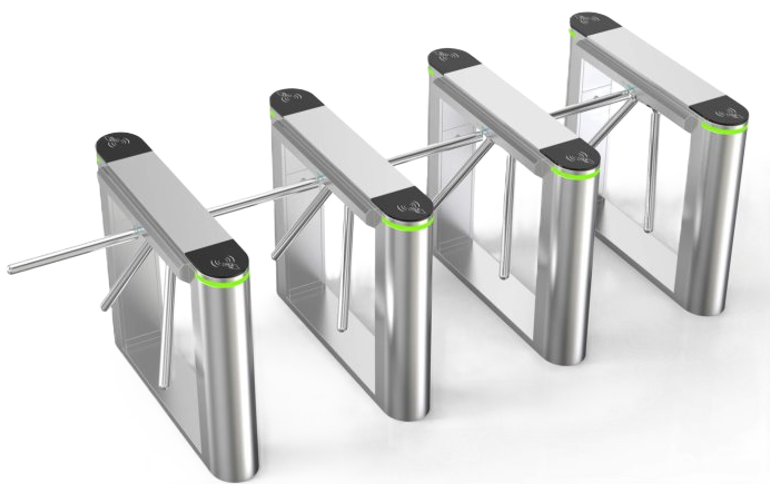
\includegraphics[width=0.7\textwidth]{fig/daosafe_turnstile.png}
    \caption{Imagen del modelo DS112 Tripod Turnstile de Daosafe.}
    \label{fig:daosafe_turnstile}
\end{figure}



Se identificó que algunos potenciales clientes de Fito App han adquirido este sistema (o similares), comprándolo directamente con el fabricante. El costo de adquisición reportado, ronda entre los \$2000 y \$2500 dólares, que incluye el torniquete y el sistema de control, para el cual se suele preferir el reconocimiento facial, aunque no es la única opción disponible. Estos gimnasios utilizan otros sistemas para la gestión administrativa, que no son compatibles con el sistema de control de acceso. Esta falta de integración entre los sistemas ha llevado a que los administradores de estos gimnasios hayan consultado a los proveedores de sus sistemas de gestión sobre la posibilidad de integrar el sistema de control de acceso, pero la respuesta ha sido negativa.

Por otro lado, los sistemas que sí se integran con el resto de la gestión del gimnasio, permiten validar no solo la identidad del usuario, sino también el estado de su membresía. Esto hace que no solo sean más seguros, sino que también permiten generar estadísticas de acceso que sean accesibles desde el mismo sistema de gestión del gimnasio. Estas características hacen que los sistemas de esta categoría sean más atractivos, y por ende, los más comunes entre los gimnasios que fueron consultados.

En esta categoría se encuentran opciones como las que ofrece la empresa \textit{Latinsoft}, con su sistema llamado \textit{Fitness 24/7 Gym} \cite{latinsoft}. Esta es una de las soluciones que tiene mayor adopción en los gimnasios medianos y grandes (ver la \textit{Tabla \ref{tab:sizes}} para entender la referencia de tamaño de un gimnasio) en el país. Para entender mejor el contexto de esta solución, se realizó una cotización directamente con un agente de ventas de dicha empresa, lo que permitió obtener información sobre sus características, precios y funcionalidades específicas. 

El producto \textit{Fitness 24/7 Gym} se ofrece como un sistema de gestión de gimnasios general que se puede obtener pagando una membresía, cuyo costo dependerá del paquete seleccionado, pero que puede ir desde los \$75 mensuales para PYMEs, hasta alrededor de  \$500 mensuales para grandes empresas y paquetes personalizados. Las funcionalidades que incluye cada paquete son variables, y no se ahondará en ellas en este documento; sin embargo, si se quiere incluir la funcionalidad de control de acceso, el gimnasio deberá asumir el costo de la compra del hardware y el sistema mecánico de acceso que deseen. En la \textit{Tabla \ref{tab:latinsoft_devices}} se muestra un resumen de los precios aproximados de los diferentes dispositivos que \textit{Latinsoft} ofrece para el control de acceso. Posteriormente, en la \textit{Tabla \ref{tab:latinsoft_mechanical}} aparecen los precios de los diferentes sistemas mecánicos que se pueden integrar con los dispositivos anteriormente mencionados.

\begin{table}[h!]
    \centering
    \begin{tabular}{c|c}
    \hline
         \textbf{Dispositivo} & \textbf{Precio aproximado}\\
         \hline
         Control por pin numérico & \$15\\
         Lector de código QR & \$90 - \$100\\
         Lector de huella dactilar & \$120\\
         Dispositivo de reconocimiento facial & \$1000 - \$1200\\
         \hline
    \end{tabular}
    \captionsetup{justification=centering}
    \caption{Precios aproximados de los dispositivos de control de acceso ofrecidos por el proveedor de \textit{Latinsoft}.}
    \label{tab:latinsoft_devices}
\end{table}

El tipo de dispositivo que es más común entre los gimnasios que utilizan este servicio es el lector de huella dactilar. Se presume que esto es por ser el sistema que utiliza datos biométricos, lo que le da un mayor nivel de seguridad al sistema, pero que también es económicamente accesible. La otra opción con esta característica es el dispositivo de reconocimiento facial, pero la diferencia de precios puede llegar a ser hasta 10 veces mayor, lo que hace que no sea una opción viable para la mayoría de los gimnasios.

Ahora bien, a partir de entrevistas realizadas a administradores de gimnasios que utilizan el sistema de \textit{Latinsoft}, se ha identificado que el lector de huella dactilar tiene un margen de error importante, lo que afecta la experiencia de los usuarios. No se ha cuantificado el porcentaje de error de los sensores de huella dactilar utilizados, pero sí se ha evidenciado un descontento general en los usuarios de estos sistemas. Desde el punto de vista de Fito App, esto representa una oportunidad de negocio si se logra implementar una solución de reconocimiento facial que sea capaz de operar de forma rápida, confiable y sin contacto físico; pero que también sea más económica que las alternativas actuales que ofrece \textit{Latinsoft}.

\begin{table}[h!]
    \centering
    \begin{tabular}{c|c}
    \hline
         \textbf{Sistema mecánico} & \textbf{Precio aproximado}\\
         \hline
         Puerta automática accionada por magnetismo & \$400 - \$500\\
         Torniquete de brazos giratorios & \$3800 - \$5000\\
         \hline
    \end{tabular}
    \captionsetup{justification=centering}
    \caption{Precios aproximados de los sistemas mecánicos de control de acceso ofrecidos por el proveedor de \textit{Latinsoft}.}
    \label{tab:latinsoft_mechanical}
\end{table}

En cuanto a los sistemas mecánicos disponibles, se sabe que estos pueden ser utilizados con cualquiera de los dispositivos de control de acceso, por lo que su escogencia pasa por considerar factores como el costo, seguridad y facilidad de instalación. Es claro que la diferencia de precio entre la opción de puerta automática y el torniquete es considerable, siendo la segunda opción hasta 10 veces más cara. Esto hace que la combinación más popular entre los clientes de \textit{Latinsoft} sea la de lector de huella dactilar con puerta automática, ya que es la opción más económica y que ofrece un nivel de seguridad aceptable.

Otra alternativa que se ha encontrado en el mercado local y que ha ganado popularidad en los últimos 2 años, es la de \textit{MNT} \cite{mnt}
. Esta es una empresa costarricense que ofrece sistemas de control de acceso para cualquier tipo de establecimiento. Recientemente, se han enfocado en el sector de gimnasios al integrar su producto con un sistema de gestión de membresías básico. Su línea de productos se enfoca principalmente en torniquetes automáticos controlados por un sistema de reconocimiento facial. En la \text{Figura \ref{fig:mnt_turnstile}} se muestra una imagen de este sistema.\footnote{Imagen promocional tomada del sitio web de MNT \cite{mnt}.}

Se utilizó la misma estrategia que con el caso anterior y se realizó una cotización directamente con un agente de ventas de \textit{MNT}. A diferencia de \textit{Fitness 24/7 Gym}, el sistema de \textit{MNT} no tiene un costo inicial de adquisición, sino que se ofrece a manera de alquiler con un costo mensual. En la \textit{Tabla \ref{tab:mnt_prices}} se resumen los precios de los paquetes ofrecidos en función de la cantidad de clientes que se manejen.

\begin{table}[h!]
    \centering
    \begin{tabular}{c|c}
    \hline
         \textbf{Cantidad de clientes} & \textbf{Costo mensual}\\
         \hline
         Hasta 300 & \$113\\
         Hasta 1500 & \$296\\
         Hasta 1500 con dos líneas de acceso & \$496\\
         Hasta 1500 solo con dispositivo de reconocimiento facial (sin torniquete) & \$78\\
         \hline
    \end{tabular}
    \captionsetup{justification=centering}
    \caption{Precios de los paquetes de sistemas de control de acceso ofrecidos por \textit{MNT}.}
    \label{tab:mnt_prices}
\end{table}

La información recopilada de la cotización con \textit{MNT} permitió concluir algunos puntos importantes. Primero, el modelo de negocio basado en un alquiler del sistema, en lugar de una sola inversión inicial elevada, puede ser de un mayor atractivo para los negocios que buscan una transición hacia estos sistemas que sea conveniente desde el punto de vista económico. En segundo lugar, se plantea la opción de solo adquirir el sistema de reconocimiento facial, sin el torniquete, lo que da lugar a cuestionarse si realmente es necesario contar con un sistema mecánico de control de acceso, o si el reconocimiento facial por sí solo es suficiente para satisfacer las necesidades de control de acceso. 

En Fito App, se plantea la hipótesis comercial de que si se combina el sistema de reconocimiento facial con una barrera de tipo psicológica, como un altavoz que emita un sonido al momento de validar el acceso, se puede lograr un efecto similar al de una barrera física, pero con un costo mucho menor. Esto representaría una ventaja competitiva importante frente a otras soluciones del mercado. La intención es que el alcance de este proyecto permita validar esta hipótesis en etapas posteriores, y que se pueda evaluar la posibilidad de ofrecerlo como una opción adicional a los gimnasios que utilicen el sistema de Fito App. 


\begin{figure}[h!]
    \centering
    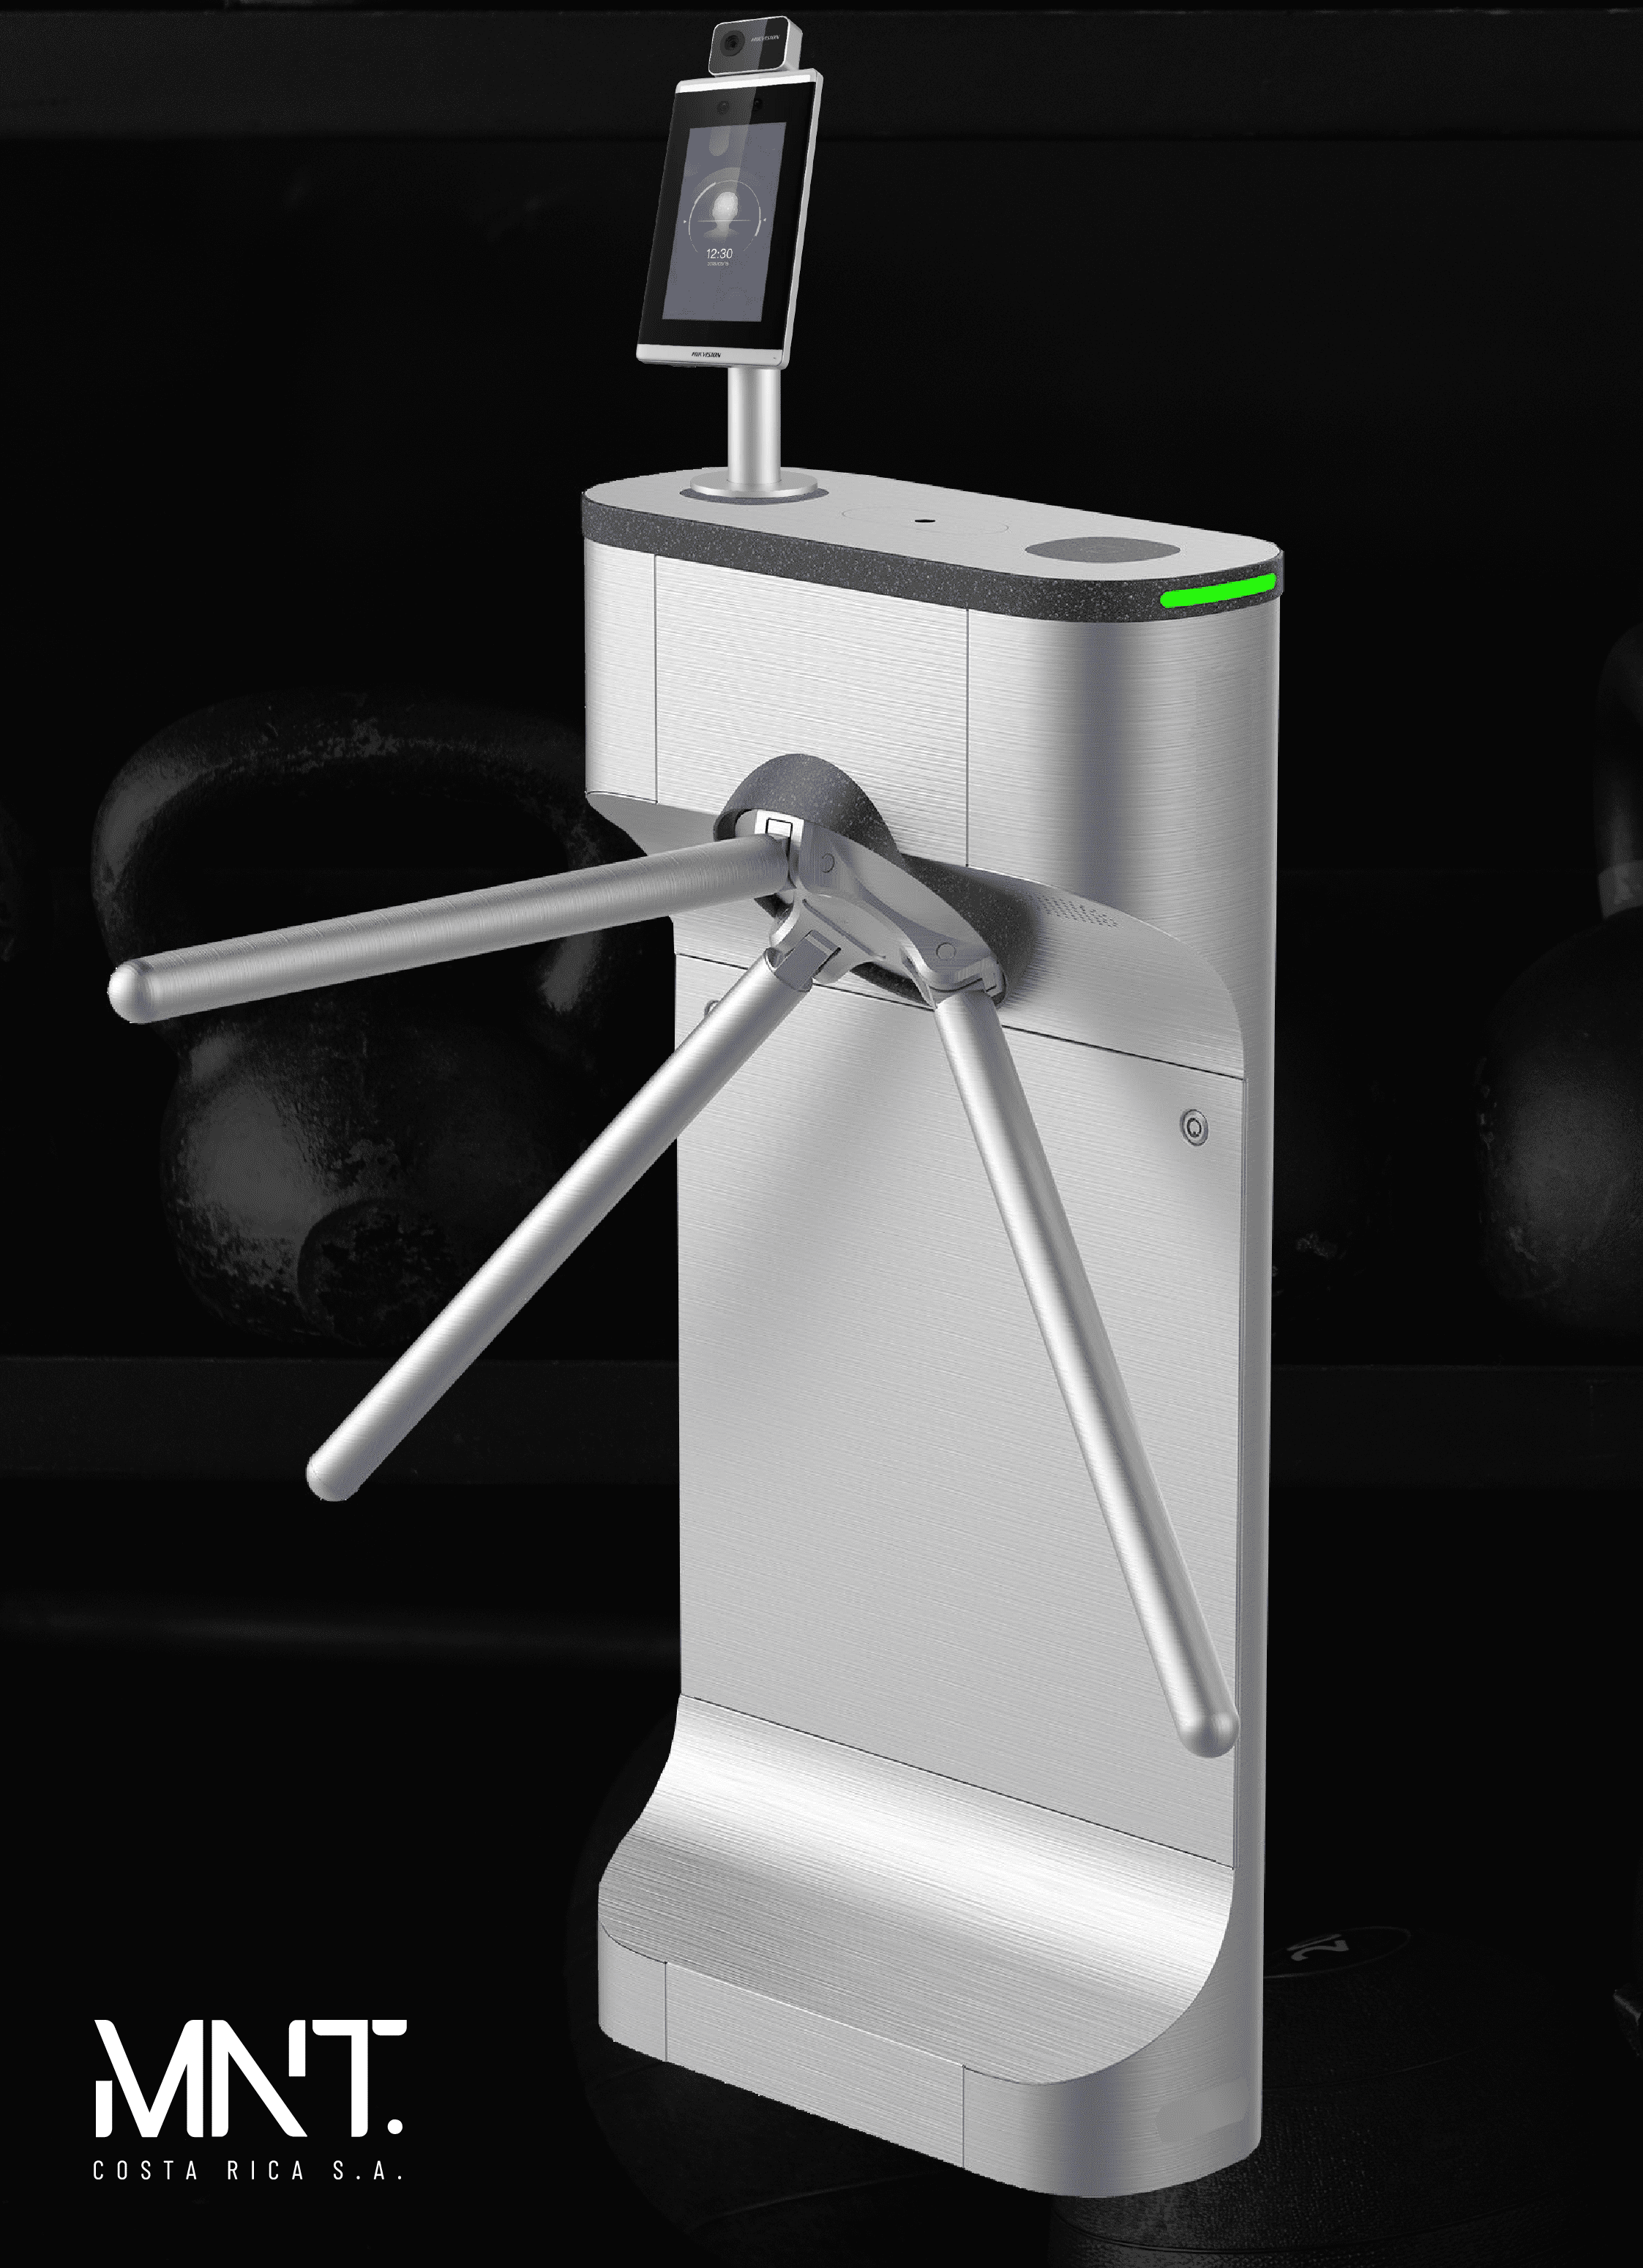
\includegraphics[width=0.4\textwidth]{fig/mnt.png}
    \caption{Imagen del sistema de control de acceso que ofrece MNT.}
    \label{fig:mnt_turnstile}
\end{figure}

\section{Planteamiento del problema}

En esta sección se describe el contexto del problema identificado y la justificación que respalda la necesidad de implementar, desde Fito App, una solución que lo aborde.

\subsection{Contexto del problema}

Como se mencionó anteriormente, Fito App desarrolla y mantiene un SaaS que le permite a la administración de los gimnasios, gestionar: sus ventas a través de membresías, las rutinas personalizadas de sus clientes y la reserva de cupos a eventos tales como clases o citas de medición. Esto mediante una aplicación web para uso de la administración del gimnasio,  y una aplicación móvil para uso de los clientes. Este fue el alcance definido para la fase de prototipado del producto y representa el estado actual de los servicios que Fito App ofrece a sus clientes.

La validación comercial del prototipo, ha arrojado resultados positivos en cuanto a la aceptación del producto; sin embargo, es sabido que el alcance del prototipo actual no es suficiente para poder competir contra otras soluciones ya establecidas en el mercado local, como lo son \textit{WStudio} \cite{wstudio} y \textit{Fitness 24/7 Gym} \cite{latinsoft}. En etapas previas a la implementación del prototipo, se condujeron investigaciones de campo en las que se entrevistó a administradores de gimnasios o centros de \textit{fitness} de diversos tipos, para poder entender mejor sus necesidades y se capturaron requerimientos importantes que principalmente son aplicables a gimnasios de dimensión mediana y grande. Para clasificar a los gimnasios por su tamaño, se utiliza la cantidad de clientes que tienen asociados. Las categorías que se identificaron de las investigaciones internas realizadas son las siguientes:

 
 \begin{table}[h!]
     \centering
     \begin{tabular}{c|c}
     \hline
          \textbf{Tamaño} & \textbf{Cantidad de clientes}\\
          \hline
          Micro & $0 < N \leq 100$\\
          Pequeño & $100 < N \leq 300$\\
          Mediano & $300 < N \leq 1000$\\
          Grande & $N > 1000$ \\
          Multi-sede &  $N > 1000$\\
          \hline
     \end{tabular}
     \caption{Categorización de los centros de \textit{fitness} según su tamaño}
     \label{tab:sizes}
 \end{table}

 El modelo de negocio por defecto de los gimnasios es utilizar la figura de membresía, la que permite que sus clientes, por un lapso determinado, tengan acceso a sus instalaciones y servicios. Así, es imprescindible que los gimnasios, principalmente los de mayor tamaño, cuenten con un \textbf{sistema de control de acceso} a sus instalaciones para poder filtrar y autorizar el ingreso únicamente de las personas que cuenten con una membresía activa. 
 
 \subsection{Justificación del problema}
 
 Tener un control activo de quiénes ingresan y salen de las instalaciones de un gimnasio es fundamental para la administración del mismo. Esto le permite no solo poder disminuir el riesgo de ingresos de personas que no hayan pagado su derecho de uso de las instalaciones (lo que representa pérdidas económicas), sino también generar estadísticas de interés con relación al flujo de clientes; como por ejemplo, la cantidad de personas que ingresan en un día, el promedio de ingresos que hay por semana, o las horas del día que tienen mayor concurrencia.

 Las estadísticas relacionadas con el flujo de ingreso de personas son valiosas para la administración porque les permite entender mejor el comportamiento de sus clientes, y a partir de ellas, tomar decisiones de negocio más informadas y basadas en datos. Ahora bien, esta información no solo es valiosa para el uso interno de la organización. Se pudo identificar del proceso de entrevistas realizadas a administradores, que también existe la necesidad de llevar el control del flujo de clientes que ingresan y salen de un local porque hay ocasiones en las que funcionarios del Ministerio de Salud de Costa Rica ejecutan auditorías o inspecciones en los gimnasios y solicitan estos datos. En caso de no brindar esta información con precisión, es posible que esto tenga repercusiones negativas de índole legal.
 
 Como es esperable, cuando un gimnasio alcanza un tamaño mediano o grande, el control de acceso deja de ser una tarea viable para un proceso manual, por lo que surge la necesidad de implementar sistemas automatizados. En el mercado local, existen varias soluciones que ofrecen sistemas de control de acceso automatizados. Las principales variantes de estos sistemas que se han encontrado son las siguientes:
 
 \begin{itemize}
     \item \textbf{Acceso con pin}: el cliente tiene asociado un pin único el cual deberá utilizar cada vez que ingrese al local, por ejemplo mediante un teclado numérico que el gimnasio pone a su disposición. Luego, el sistema evalúa si corresponde a un cliente con una membresía activa. Es una solución de bajo costo, pero tiene la desventaja de que su seguridad puede ser sorteada fácilmente si un usuario comparte su pin a otra persona sin autorización de ingreso. También puede ser un inconveniente para usuarios olvidadizos que les cueste trabajo memorizar el código.
     
     \item \textbf{Acceso con código QR}: el funcionamiento es similar al acceso por pin, ya que el usuario debe mostrar el código QR cada vez que ingresa al local. Es una solución que se popularizó durante la pandemia ya que evita el contacto físico directo con algún medio compartido. La lectura se puede hacer con un dispositivo específico o con un dispositivo móvil, de forma eficaz y rápida, con muy poco margen de error. Tiene la misma desventaja que el punto anterior de la posibilidad de compartir el código de forma deshonesta.
     
     \item \textbf{Lector de huella dactilar}: es una de las soluciones más populares actualmente. Tiene la gran ventaja de utilizar datos bio-métricos para el acceso, por lo que se eliminan los problemas de seguridad de las dos soluciones anteriores. Aunque tiene la desventaja de que hay un cierto margen de error en el sistema, que tiende a arrojar falsos negativos, y que ha afectado la experiencia de los usuarios a los que se les ha consultado. No se ha cuantificado el porcentaje de error de los sensores de huella dactilares utilizados, pero sí se ha evidenciado un descontento general en los usuarios de estos sistemas. Otro punto negativo es el contacto que podría generar un foco de contagio sino se tienen medidas adecuadas de higiene al tocar el dispositivo.
     
     \item \textbf{Reconocimiento facial}: es una solución innovadora que está ganando popularidad en los sistemas de control de acceso en general. Al igual que el lector de huella dactilar, utiliza datos bio-métricos, lo que favorece la seguridad del sistema, aunque esta solución utiliza tecnología de reconocimiento de patrones que garantizan un mayor porcentaje de acierto que los sensores de huella, que pueden perder precisión si se ensucian o se ven afectados por la humedad característica de lugares como los gimnasios. También, al evitar el contacto físico, el reconocimiento facial se coloca como una alternativa más segura para la salud de las personas evitando focos de contagio de enfermedades. Ahora bien, se ha identificado que soluciones de este tipo que ofrecen otros SaaS similares al de Fito App, tienen problemas de rendimiento y presentan latencias elevadas a la hora de procesar las solicitudes de acceso, afectando de manera importante la experiencia de usuario. También, esta se suele presentar como la alternativa de mayor costo económico, lo que puede llevar a que centro de \textit{fitness} prefieran otro tipo de soluciones más accesibles. En Fito App, esto se interpreta como una oportunidad de negocio si se logra implementar una solución más eficiente y de menor costo que las alternativas actuales en el país.

 \end{itemize}

 \subsection{Enunciado del problema}

En síntesis, el proyecto busca atacar el problema de los ingresos no autorizados a los gimnasios, que afecta negativamente la seguridad y la experiencia de los usuarios que sí tienen membresías activas, así como los réditos económicos de la administración. Esto mediante un sistema automatizado que controle y registre el acceso de los usuarios a los diferentes centros de \textit{fitness}, los cuales son potenciales clientes de Fito App, lo que permitiría robustecer el producto actual y colocarlo como una alternativa más competente en el mercado local. 

Dicho esto, se considera que una solución de reconocimiento facial que sea capaz de operar de forma rápida, confiable y sin contacto físico, mejorando la seguridad y comodidad para los usuarios, le daría una ventaja competitiva al producto. El desarrollo del producto descrito en este documento busca desarrollar un sistema de bajo costo, que minimice la latencia en el procesamiento de reconocimiento facial y se integre eficientemente con el sistema de gestión de membresías de Fito App, con un enfoque en la mantenibilidad y escalabilidad, aumentando así su competitividad en el mercado y su valor para los gimnasios que tengan dicha necesidad.

\section{Objetivos del proyecto}
En este apartado se definen los objetivos del proyecto, tanto el objetivo general como los específicos. 

% Recordar que todos los objetivos deben contener el qué, el para y el cómo

\subsection{Objetivo general}
% El objetivo general responde de manera directa el problema en concreto
Desarrollar un sistema de control de acceso para gimnasios, que mejore la seguridad y eficiencia en la validación de membresías en el sistema de gestión de Fito App, utilizando una plataforma de \textit{hardware} embebido. % con un sistema operativo personalizado y de propósito específico. %para garantizar la optimización de recursos y la integración con el sistema de gestión de Fito App.


\subsection{Objetivos específicos}\label{secc:objectives}
Los objetivos específicos se asocian con un identificador único para poder ser referenciados en secciones posteriores del documento con mayor facilidad.

\begin{enumerate}
    \item \textbf{OE1}: Diseñar la arquitectura de un sistema embebido de control de acceso, %para establecer una estructura clara de hardware y software 
    que permita la captura y análisis de datos biométricos, mediante el uso de una plataforma de bajo costo con un sistema operativo de propósito específico.

    \item \textbf{OE2}: Desarrollar un módulo de reconocimiento facial, para la validación de la identidad de los usuarios en el punto de ingreso al gimnasio, mediante la integración de una cámara y el uso de servicios en la nube. %que posibiliten el procesamiento y análisis de imágenes en tiempo real.
    
    \item \textbf{OE3}: Integrar un módulo de reportes en el sistema de administración de Fito App, %para que los administradores de gimnasios puedan 
    que permita la consulta de estadísticas de acceso de los usuarios, mediante %una interfaz de comunicación entre el sistema de reconocimiento facial y el \textit{backend} de Fito App, así como la visualización de los datos a través de una interfaz web.
    una interfaz web.
    
    \item \textbf{OE4}: Evaluar el rendimiento del sistema en un entorno real, para la verificación del cumplimiento de los requisitos de latencia, precisión y experiencia de usuario, mediante pruebas de campo controladas. % que midan la latencia, la tasa de aciertos en el reconocimiento facial y la confiabilidad operativa del sistema.

\end{enumerate}

\newpage
\section{Alcances, entregables y limitaciones del proyecto.}
En esta sección se describen los alcances, entregables y limitaciones del proyecto, con el objetivo de delimitar claramente lo que se espera lograr, los productos que se generarán como resultado del desarrollo y las restricciones que podrían influir en la ejecución del mismo.

\subsection{Alcances}
El proyecto contempla el diseño, implementación e integración de un sistema de control de acceso para gimnasios, utilizando reconocimiento facial como método de validación de identidad. El sistema será desarrollado sobre una plataforma embebida de propósito específico, conectada a servicios de reconocimiento facial en la nube, y comunicada con el sistema administrativo actual de Fito App.

El alcance del proyecto incluye:
\begin{itemize}
    \item El diseño e implementación de la arquitectura de hardware y software del sistema embebido, incluyendo su sistema operativo personalizado.
    \item El desarrollo del módulo de captura y reconocimiento facial para validación de acceso.
    \item La implementación de un mecanismo de retroalimentación auditiva y visual para el usuario al momento de validar su acceso.
    \item La integración con el \textit{backend} de Fito App para registrar accesos y generar estadísticas.
    \item La integración de un módulo de reportes en la aplicación web de Fito App, que permita a los administradores consultar los registros de acceso.
    \item La ejecución de pruebas de validación funcional y de rendimiento en un entorno real de operación.
\end{itemize}

El proyecto no contempla el desarrollo de modelos de reconocimiento facial propios, ya que se utilizarán servicios preexistentes. Tampoco se considera como parte del alcance la integración con mecanismos físicos de cierre o apertura de acceso, tales como puertas o torniquetes; el enfoque se centra en la validación y registro digital del acceso y en una retroalimentación adecuada al usuario.

\subsection{Entregables}
En la \textit{Tabla \ref{tab:deliverables}}, se resumen los entregables del proyecto en función de los objetivos específicos planteados.

\begin{table}[h!]
    \centering
    \begin{tabular}{p{1.5cm}|p{4.5cm}|p{8cm}}
        \hline
        \textbf{Obj.} & \textbf{Entregable} & \textbf{Descripción} \\ \hline
        \textbf{OE1} & Documento de arquitectura & Especificación de la arquitectura hardware-software del sistema embebido, incluyendo diagramas y justificación técnica. \\ \hline
        \textbf{OE2} & Módulo de reconocimiento facial & Aplicación funcional que capture imágenes, valide identidades mediante un servicio de reconocimiento facial y brinde retroalimentación al usuario por medio de señales auditivas (buzzer) y visuales (pantalla). \\ \hline
        \textbf{OE3} & Módulo de reportes & Interfaz de visualización web integrada al sistema de Fito App para mostrar estadísticas de acceso a los administradores. \\ \hline
        \textbf{OE4} & Informe de pruebas de rendimiento & Documento con los resultados de pruebas realizadas en entorno real, incluyendo métricas de latencia y precisión. \\ \hline
    \end{tabular}
    \caption{Entregables del proyecto según objetivo específico}
    \label{tab:deliverables}
\end{table}


\subsection{Limitaciones del proyecto}
El desarrollo del proyecto se verá influenciado por diversas limitaciones que podrían afectar su ejecución y resultados. A continuación se enumeran las principales limitaciones identificadas:

\begin{enumerate}
    \item La ejecución del proyecto deberá hacerse en un lapso de 16 semanas, es decir, un semestre lectivo del ITCR, planteado para iniciarse el 10 de febrero del 2025.
    \item La organización cuenta con un dispositivo \textit{Raspberry Pi 4 Model B}, del cual se dispone para el desarrollo del proyecto de ser necesario. El resto de componentes del sistema deberán ser adquiridos externamente. En la etapa de diseño deberá de tomarse la decisión sobre la plataforma de \textit{hardware} y componentes que se utilizará.
    \item Es posible que adquisición del \textit{hardware} necesario para el proyecto implique hacer una compra internacional, lo que supone una limitación en cuanto al tiempo de latencia asociado al proceso de envío y entrega de los productos.
    \item La organización cuenta con un presupuesto limitado para la ejecución del proyecto, lo que podría restringir la adquisición de ciertos componentes o servicios necesarios para el desarrollo del sistema.
    \item Los entregables generados por el proyecto, como código fuente y documentación, serán de carácter confidencial y propiedad intelectual de Fito App.
    \item Las pruebas de funcionalidad completa podrían estar limitadas por la disponibilidad de un gimnasio dispuesto a colaborar, lo cual podría restringir el número y la duración de las pruebas en un entorno real.
\end{enumerate}


%\index{objetivos}

%%% Local Variables: 
%%% mode: latex
%%% TeX-master: "main"
%%% End: 
